% Bias & Variance --- detailed deep-dive deck (frequentist view of a frozen PFN).
% Standalone mini-deck, same metropolis style as ../presentation.tex.
% Build with: make   (tectonic)
\documentclass[aspectratio=169,10pt]{beamer}

\usetheme{metropolis}
\metroset{progressbar=frametitle, numbering=fraction, block=fill}

\usepackage[T1]{fontenc}
\usepackage{booktabs}
\usepackage{amsmath,amssymb}
\usepackage{tikz}
\usetikzlibrary{positioning,arrows.meta,fit,backgrounds,calc,matrix}
\usepackage{pgfplots}
\pgfplotsset{compat=1.18}
\usepackage{xcolor}

% --- palette (identical to the main deck) ----------------------------------
\definecolor{accent}{HTML}{C1121F}
\definecolor{ink}{HTML}{2B2D42}
\definecolor{muted}{HTML}{6C757D}
\definecolor{good}{HTML}{2A9D8F}
\setbeamercolor{frametitle}{bg=ink}
\setbeamercolor{background canvas}{bg=white}
\setbeamercolor{normal text}{fg=ink, bg=white}
\setbeamercolor{progress bar}{fg=accent}
\setbeamercolor{alerted text}{fg=accent}

\newcommand{\hl}[1]{{\color{accent}\textbf{#1}}}
\newcommand{\gd}[1]{{\color{good}\textbf{#1}}}
\newcommand{\mut}[1]{{\color{muted}#1}}
\newcommand{\cit}[1]{{\scriptsize\color{muted}[#1]}}

% --- reusable dartboard: \board{shift}{label}{dart-list} -------------------
% draws 3 rings + green bullseye at its own origin; darts are accent dots.
\tikzset{ring/.style={draw=muted,line width=0.4pt}}
\newcommand{\board}[3]{%
  \begin{scope}[shift={#1}]
    \draw[ring](0,0)circle(0.8);\draw[ring](0,0)circle(0.53);\draw[ring](0,0)circle(0.27);
    \foreach \dx/\dy in {#3} \fill[accent](\dx,\dy)circle(0.05);
    \draw[good,line width=0.8pt](-0.1,0)--(0.1,0)(0,-0.1)--(0,0.1);
    \node[font=\footnotesize, align=center] at (0,-1.15){#2};
  \end{scope}}

\title{Bias and Variance}
\subtitle{the frequentist view of a frozen PFN \;\cit{Nagler '23, \S5}}
\author{\underline{Gurmeher} Singh Puri \;\&\; Salih \underline{Bora} Öztürk}
\institute{Group 4 \;\textperiodcentered\; FM4SD Seminar \;\textperiodcentered\; SS26}
\date{}

\begin{document}

\maketitle

% ===========================================================================
% 1. The reframe + the decomposition
% ===========================================================================
\begin{frame}[t]{The reframe: a frozen PFN is just an estimator}

  \onslide<1->{\centering
    Forget where it came from. Treat the frozen $q_{\hat\theta}$ as an \hl{ordinary estimator}
    of the truth $p_0(y\mid x)$: data in, prediction out.\par}
  \vfill

  \onslide<2->{\centering
  $\displaystyle
    \underbrace{q_{\hat\theta} - p_0}_{\textstyle\text{error}}
    \;=\;
    \underbrace{q_{\hat\theta} - \mathbb{E}[q_{\hat\theta}]}_{\textstyle\color{accent}\text{variance}}
    \;+\;
    \underbrace{\mathbb{E}[q_{\hat\theta}] - p_0}_{\textstyle\color{ink}\text{bias}}
  $\par}
  \smallskip
  \onslide<2->{\centering
    {\footnotesize\mut{$q_{\hat\theta}=q_{\hat\theta}(y\mid x,\mathcal D_n)$;\quad
    $\mathbb{E}$ averages over random datasets $\mathcal D_n\sim p_0^{\,n}$.}}\par}
  \vfill

  \onslide<3->{\centering
    The only random thing is the \hl{data} $\mathcal D_n$ --- the network is fixed.\\
    So the prediction is random, and its error splits the classic way.\par}
  \vfill
\end{frame}

% ===========================================================================
% 2. The dartboard metaphor
% ===========================================================================
\begin{frame}[t]{The picture: a dartboard}

  \onslide<1->{\centering
    Each \hl{dart} $=$ the prediction from \emph{one} random dataset.\quad
    The \gd{bullseye} $=$ the truth $p_0$.\par}
  \vfill

  \onslide<2->{\centering
  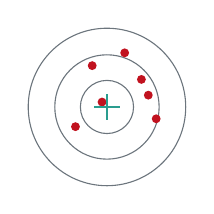
\begin{tikzpicture}[>=Latex, scale=1.25]
    \draw[ring](0,0)circle(0.8);\draw[ring](0,0)circle(0.53);\draw[ring](0,0)circle(0.27);
    \foreach \dx/\dy in {0.35/0.28,-0.15/0.42,0.5/-0.12,-0.32/-0.2,0.18/0.55,-0.05/0.05,0.42/0.12}
      \fill[accent](\dx,\dy)circle(0.045);
    \draw[good,line width=1pt](-0.13,0)--(0.13,0)(0,-0.13)--(0,0.13);
  \end{tikzpicture}}
  \vfill

  \onslide<3->{\centering
    Hand the \emph{same} predictor a fresh random dataset $\Rightarrow$ a slightly different dart.\\
    Many datasets $\Rightarrow$ a \hl{cluster} of darts. Two things can go wrong, independently:\\[2pt]
    {\footnotesize\mut{how \emph{scattered} the cluster is \,(variance)\quad and\quad
    how far its \emph{centre} sits from the bullseye \,(bias).}}\par}
  \vfill
\end{frame}

% ===========================================================================
% 3. Variance = scatter
% ===========================================================================
\begin{frame}[t]{Variance $=$ scatter}

  \onslide<1->{\centering
    {\color{accent}\textbf{Variance}} $=\ q_{\hat\theta}-\mathbb{E}[q_{\hat\theta}]$:
    how much the dart \hl{moves} just because you got a \emph{different} random dataset.\par}
  \vfill

  \onslide<2->{\centering
  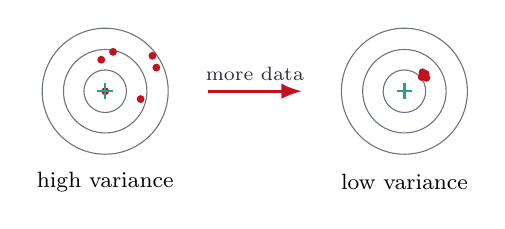
\begin{tikzpicture}[>=Latex]
    \board{(0,0)}{high variance}{0.6/0.45,-0.05/0.4,0.45/-0.1,0.0/0.0,0.65/0.3,0.1/0.5}
    \draw[->,line width=1pt,accent] (1.3,0)--(2.5,0)
      node[midway,above,font=\scriptsize,text=ink]{more data};
    \board{(3.8,0)}{low variance}{0.27/0.22,0.22/0.18,0.28/0.17,0.23/0.24,0.26/0.2,0.24/0.21}
  \end{tikzpicture}}
  \vfill

  \onslide<3->{\centering
    \gd{Key fact:} variance \hl{shrinks as $n$ grows} --- more data pulls the darts together.\\[2pt]
    {\footnotesize\mut{(the cluster's \emph{centre} does not move --- that leftover offset is bias.)}}\par}
  \vfill
\end{frame}

% ===========================================================================
% 4. Bias = offset
% ===========================================================================
\begin{frame}[t]{Bias $=$ offset}

  \onslide<1->{\centering
    {\color{ink}\textbf{Bias}} $=\ \mathbb{E}[q_{\hat\theta}]-p_0$:
    how far the cluster's \hl{centre} sits from the bullseye --- a \emph{systematic} error.\par}
  \vfill

  \onslide<2->{\centering
  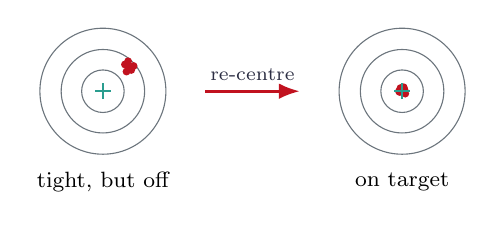
\begin{tikzpicture}[>=Latex]
    \board{(0,0)}{tight, but off}{0.33/0.30,0.28/0.34,0.36/0.27,0.30/0.25,0.39/0.32,0.32/0.38}
    \draw[->,line width=1pt,accent] (1.3,0)--(2.5,0)
      node[midway,above,font=\scriptsize,text=ink]{re-centre};
    \board{(3.8,0)}{on target}{0.03/0.02,-0.02/0.04,0.04/-0.03,-0.03/-0.01,0.02/0.05,-0.04/0.0}
  \end{tikzpicture}}
  \vfill

  \onslide<3->{\centering
    \hl{Bias does not shrink with more data.} A tight cluster in the wrong place is still wrong.\\[2pt]
    {\footnotesize\mut{more data makes a biased predictor \emph{tighter}, not \emph{truer}.}}\par}
  \vfill
\end{frame}

% ===========================================================================
% 5. The 2x2 grid
% ===========================================================================
\begin{frame}[t]{The four shooters}

  \onslide<1->{\centering Columns $=$ variance (scatter)\quad\textperiodcentered\quad rows $=$ bias (offset).\par}
  \vfill

  \onslide<1->{\centering
  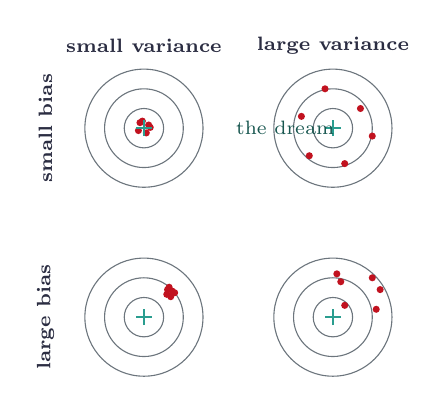
\begin{tikzpicture}[scale=1.0,
      ring/.style={draw=muted, line width=0.4pt}, dart/.style={fill=accent, draw=none},
      hdr/.style={font=\scriptsize\bfseries, text=ink}]
    \foreach \cx/\cy in {0/0, 2.4/0, 0/-2.4, 2.4/-2.4}{%
      \draw[ring] (\cx,\cy) circle(0.75); \draw[ring] (\cx,\cy) circle(0.50); \draw[ring] (\cx,\cy) circle(0.25);}
    \foreach \dx/\dy in {0.06/0.04,-0.05/0.07,0.03/-0.06,-0.07/-0.03,0.08/0.01,-0.02/0.09}
      \fill[dart] (\dx,\dy) circle(0.045);
    \foreach \dx/\dy in {0.35/0.25,-0.4/0.15,0.15/-0.45,-0.3/-0.35,0.5/-0.1,-0.1/0.5}
      \fill[dart] ({2.4+\dx},{\dy}) circle(0.045);
    \foreach \dx/\dy in {0.36/0.33,0.30/0.35,0.34/0.26,0.29/0.29,0.39/0.31,0.32/0.38}
      \fill[dart] ({\dx},{-2.4+\dy}) circle(0.045);
    \foreach \dx/\dy in {0.5/0.5,0.1/0.45,0.55/0.1,0.15/0.15,0.6/0.35,0.05/0.55}
      \fill[dart] ({2.4+\dx},{-2.4+\dy}) circle(0.045);
    \foreach \cx/\cy in {0/0, 2.4/0, 0/-2.4, 2.4/-2.4}{%
      \draw[good, line width=0.7pt] (\cx-0.10,\cy)--(\cx+0.10,\cy) (\cx,\cy-0.10)--(\cx,\cy+0.10);}
    \node[hdr] at (0,1.05) {small variance};   \node[hdr] at (2.4,1.05) {large variance};
    \node[hdr, rotate=90] at (-1.25,0) {small bias};  \node[hdr, rotate=90] at (-1.25,-2.4) {large bias};
    \node[good!55!black, font=\scriptsize, anchor=west] at (1.0,0.0) {\,the dream};
  \end{tikzpicture}}
  \vfill

  \onslide<2->{\centering {\gd{Want top-left:}} small bias \emph{and} small variance.\par}
\end{frame}

% ===========================================================================
% 6. Squared-error (MSE) decomposition
% ===========================================================================
\begin{frame}[t]{One dart, two errors: $\text{MSE}=\text{bias}^2+\text{variance}$}

  \begin{columns}[c]
    \column{0.46\textwidth}
      \onslide<1->{\centering
      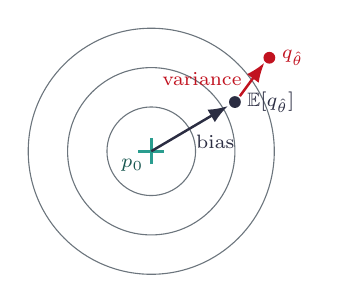
\begin{tikzpicture}[>=Latex, scale=1.25]
        \draw[ring](0,0)circle(1.25);\draw[ring](0,0)circle(0.85);\draw[ring](0,0)circle(0.45);
        \draw[good,line width=1pt](-0.13,0)--(0.13,0)(0,-0.13)--(0,0.13);
        \node[good!55!black, font=\scriptsize, below left=-1pt] at (0,0){$p_0$};
        \fill[ink] (0.85,0.5) circle(0.06);
        \node[ink, font=\scriptsize, right=1pt] at (0.85,0.5){$\mathbb E[q_{\hat\theta}]$};
        \fill[accent] (1.2,0.95) circle(0.06);
        \node[accent, font=\scriptsize, right=1pt] at (1.2,0.95){$q_{\hat\theta}$};
        \draw[->, ink, line width=0.9pt] (0,0) -- (0.78,0.46)
          node[midway, below right=-2pt, font=\scriptsize]{bias};
        \draw[->, accent, line width=0.9pt] (0.9,0.56) -- (1.15,0.9)
          node[midway, left=0pt, font=\scriptsize]{variance};
      \end{tikzpicture}}
    \column{0.54\textwidth}
      \onslide<2->{The expected squared error splits exactly:
        \[ \mathbb{E}\big[(q_{\hat\theta}-p_0)^2\big]
           = \underbrace{(\mathbb{E}[q_{\hat\theta}]-p_0)^2}_{\textstyle\color{ink}\text{bias}^2}
           + \underbrace{\mathbb{E}\big[(q_{\hat\theta}-\mathbb{E}[q_{\hat\theta}])^2\big]}_{\textstyle\color{accent}\text{variance}}. \]}
      \medskip
      \onslide<3->{{\footnotesize\mut{The cross-term vanishes because $\mathbb E[q_{\hat\theta}-\mathbb E[q_{\hat\theta}]]=0$ ---
        bias and variance are \emph{orthogonal} (a Pythagorean split).}}\par}
  \end{columns}
\end{frame}

% ===========================================================================
% 7. Why it matters + the plan
% ===========================================================================
\begin{frame}[t]{Why this split runs the rest of the talk}

  \onslide<1->{\centering
    More data shrinks \hl{variance}, never \hl{bias} --- so the two halves need \emph{different} tools.\par}
  \vfill

  \begin{columns}[T]
    \column{0.5\textwidth}
      \onslide<2->{\begin{block}{Variance \;\normalfont\small\mut{the easy half}}
        \footnotesize Falls almost \gd{for free} from the architecture:
        \emph{symmetry} \cit{Lem 5.1} $+$ \emph{diminishing sensitivity} \cit{Thm 5.2}
        $\Rightarrow$ variance $\to 0$ at rate $1/n$.
      \end{block}}
    \column{0.5\textwidth}
      \onslide<3->{\begin{block}{Bias \;\normalfont\small\mut{the hard half}}
        \footnotesize No free lunch. Vanishing bias \emph{requires} \hl{locality} \cit{Thm 5.4};
        a plain transformer isn't local, so its bias \emph{plateaus}.
      \end{block}}
  \end{columns}
  \vfill

  \onslide<4->{\centering
    {\footnotesize In TabPFN \cit{Fig.\ 1}: variance keeps falling $\sim 1/n$, but bias
    \hl{flattens around $n\approx1000$} --- exactly this picture.}\par}
  \vfill
\end{frame}

\end{document}
